% Column-width, editable TikZ. Panel captions are below plots.
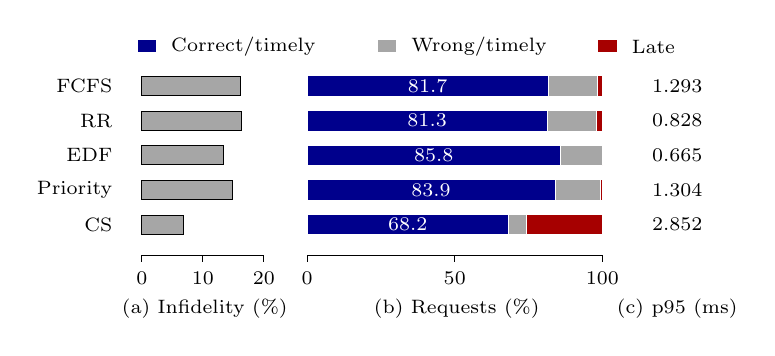
\begin{tikzpicture}[font=\scriptsize]
\fill[blue!55!black] (1.1,3.33) rectangle (1.33,3.48);\node[anchor=west] at (1.4000000000000001,3.4) {Correct/timely};
\fill[black!35] (4.15,3.33) rectangle (4.380000000000001,3.48);\node[anchor=west] at (4.45,3.4) {Wrong/timely};
\fill[red!65!black] (6.95,3.33) rectangle (7.180000000000001,3.48);\node[anchor=west] at (7.25,3.4) {Late};
\node[anchor=east] at (0.9,2.9) {FCFS};
\filldraw[fill=black!35,draw=black,line width=.25pt] (1.15,2.78) rectangle (2.4041140965932026,3.02);
\filldraw[fill=blue!55!black,draw=white,line width=.2pt] (3.25,2.77) rectangle (6.3119049072265625,3.03);
\node[text=white] at (4.780952453613281,2.9) {81.7};
\filldraw[fill=black!35,draw=white,line width=.2pt] (6.3119049072265625,2.77) rectangle (6.933013916015625,3.03);
\filldraw[fill=red!65!black,draw=white,line width=.2pt] (6.933013916015625,2.77) rectangle (7.0,3.03);
\node[] at (7.95,2.9) {1.293};
\node[anchor=east] at (0.9,2.46) {RR};
\filldraw[fill=black!35,draw=black,line width=.25pt] (1.15,2.34) rectangle (2.409689214666371,2.58);
\filldraw[fill=blue!55!black,draw=white,line width=.2pt] (3.25,2.33) rectangle (6.298286437988281,2.59);
\node[text=white] at (4.774143218994141,2.46) {81.3};
\filldraw[fill=black!35,draw=white,line width=.2pt] (6.298286437988281,2.33) rectangle (6.917793273925781,2.59);
\filldraw[fill=red!65!black,draw=white,line width=.2pt] (6.917793273925781,2.33) rectangle (7.0,2.59);
\node[] at (7.95,2.46) {0.828};
\node[anchor=east] at (0.9,2.02) {EDF};
\filldraw[fill=black!35,draw=black,line width=.25pt] (1.15,1.9) rectangle (2.1844986432588067,2.14);
\filldraw[fill=blue!55!black,draw=white,line width=.2pt] (3.25,1.8900000000000001) rectangle (6.468574523925781,2.15);
\node[text=white] at (4.859287261962891,2.02) {85.8};
\filldraw[fill=black!35,draw=white,line width=.2pt] (6.468574523925781,1.8900000000000001) rectangle (7.0,2.15);
\filldraw[fill=red!65!black,draw=white,line width=.2pt] (7.0,1.8900000000000001) rectangle (7.0,2.15);
\node[] at (7.95,2.02) {0.665};
\node[anchor=east] at (0.9,1.5799999999999998) {Priority};
\filldraw[fill=black!35,draw=black,line width=.25pt] (1.15,1.46) rectangle (2.29614075705958,1.6999999999999997);
\filldraw[fill=blue!55!black,draw=white,line width=.2pt] (3.25,1.4499999999999997) rectangle (6.396629333496094,1.71);
\node[text=white] at (4.823314666748047,1.5799999999999998) {83.9};
\filldraw[fill=black!35,draw=white,line width=.2pt] (6.396629333496094,1.4499999999999997) rectangle (6.975471496582031,1.71);
\filldraw[fill=red!65!black,draw=white,line width=.2pt] (6.975471496582031,1.4499999999999997) rectangle (7.0,1.71);
\node[] at (7.95,1.5799999999999998) {1.304};
\node[anchor=east] at (0.9,1.14) {CS};
\filldraw[fill=black!35,draw=black,line width=.25pt] (1.15,1.02) rectangle (1.6840436183407197,1.2599999999999998);
\filldraw[fill=blue!55!black,draw=white,line width=.2pt] (3.25,1.0099999999999998) rectangle (5.807487487792969,1.27);
\node[text=white] at (4.528743743896484,1.14) {68.2};
\filldraw[fill=black!35,draw=white,line width=.2pt] (5.807487487792969,1.0099999999999998) rectangle (6.0279388427734375,1.27);
\filldraw[fill=red!65!black,draw=white,line width=.2pt] (6.0279388427734375,1.0099999999999998) rectangle (7.0,1.27);
\node[] at (7.95,1.14) {2.852};
\draw[thin] (1.15,.75)--(2.7,.75);\draw (1.15,.75)--(1.15,.67);\node[] at (1.15,0.46) {0};
\draw (1.9249999999999998,.75)--(1.9249999999999998,.67);\node[] at (1.9249999999999998,0.46) {10};
\draw (2.7,.75)--(2.7,.67);\node[] at (2.7,0.46) {20};
\draw[thin] (3.25,.75)--(7.0,.75);\draw (3.25,.75)--(3.25,.67);\node[] at (3.25,0.46) {0};
\draw (5.125,.75)--(5.125,.67);\node[] at (5.125,0.46) {50};
\draw (7.0,.75)--(7.0,.67);\node[] at (7.0,0.46) {100};
\node[] at (1.95,0.07) {(a) Infidelity (\%)};
\node[] at (5.15,0.07) {(b) Requests (\%)};
\node[] at (7.95,0.07) {(c) p95 (ms)};
\end{tikzpicture}
